\chapter{Tribal NeuroSim -- Futtatások, validáció és értelmezés}

\section{Világ-mechanikák}

A szimuláció terét egy hexagonális rács alkotja. A flexset adatkészletből inicializált futtatások $\approx$36\,100 tile-os térképen játszódnak; a soloq futtatások kisebb világokat kapnak. Minden tile-hoz egy biome-típus van rendelve (DenseForest, Riverland, DrySteppe, Mountains, Marsh, Cold), amely meghatározza az alap élelmiszertermelési rátát.

A polity-szintek és fejlődési feltételek, a harci mechanika (Poisson-modell), az iteratív újratervezési döntések és a liveness-fix részletei a kibővített verzió 15. fejezetében találhatók.

\section{Kísérleti futtatási narratívák}

A négy teljes kísérleti futtatás összefoglalója:

\begin{table}[h]
\centering
\small
\caption{A négy záró Tribal NeuroSim futtatás összehasonlítása}
\label{tab:neurosim-run-comparison-final}
\resizebox{\textwidth}{!}{%
\begin{tabular}{llllllll}
\hline
\textbf{Futtatás} & \textbf{Adatkészlet} & \textbf{Seed} & \textbf{Győztes} & \textbf{Viselkedés} & \textbf{Agresszió} & \textbf{Migráció} & \textbf{Végső tick} \\
\hline
run67fl7777 & Flexset & 7777 & Tribe 355 & Warband/Combat & 0{,}18 & 0{,}88 & 2538 \\
run67fl42 & Flexset & 42 & Tribe 596 & Warband/Combat & 0{,}13 & 0{,}87 & 2487 \\
run67sq42 & SoloQ & 42 & Tribe 89 & Vanguard/Risk & 0{,}11 & 0{,}16 & 2046 \\
run67sq7777 & SoloQ & 7777 & Tribe 70 & Supply/Resource & 0{,}68 & 0{,}87 & 2541 \\
\hline
\end{tabular}
}
\end{table}

\begin{figure}[H]
\centering
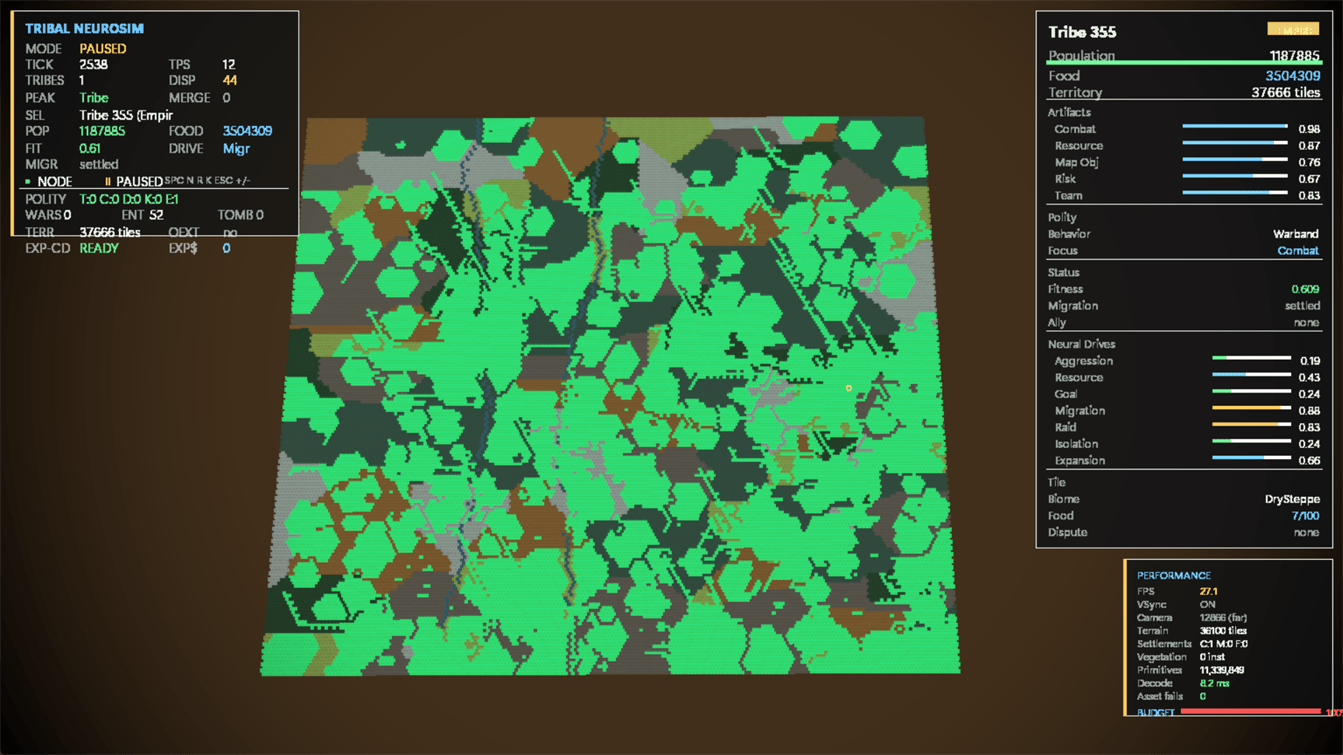
\includegraphics[width=0.9\textwidth]{assets/neurosim/run67fl7777-fl-s7777-tick2538-last.png}
\caption{Flexset, seed=7777, tick=2538: Tribe 355 (Warband/Combat) győzelme, 37\,666 tile-os végső területtel.}
\end{figure}

\begin{figure}[H]
\centering
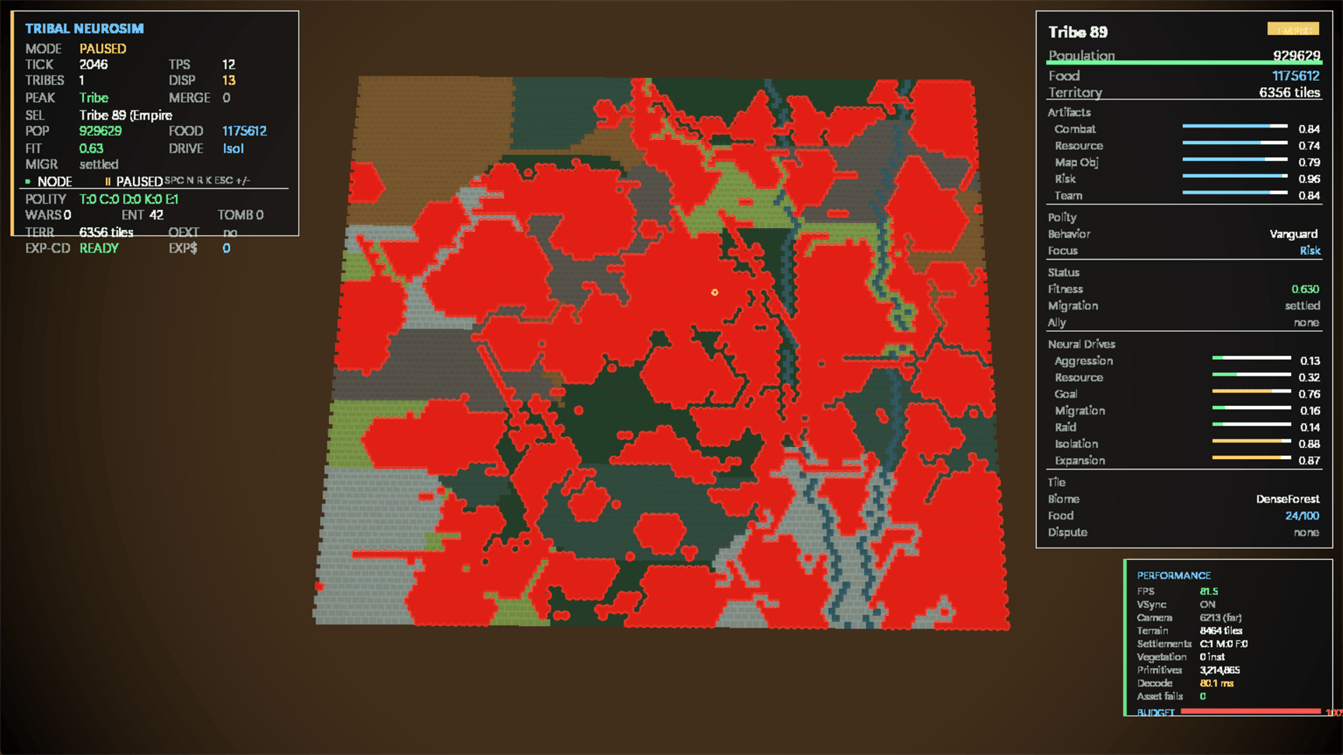
\includegraphics[width=0.9\textwidth]{assets/neurosim/run67sq42-sq-s42-tick2046-last.png}
\caption{SoloQ, seed=42, tick=2046: Tribe 89 (Vanguard/Risk) győzelme, 6\,356 tile-os végső területtel.}
\end{figure}

\begin{figure}[H]
\centering
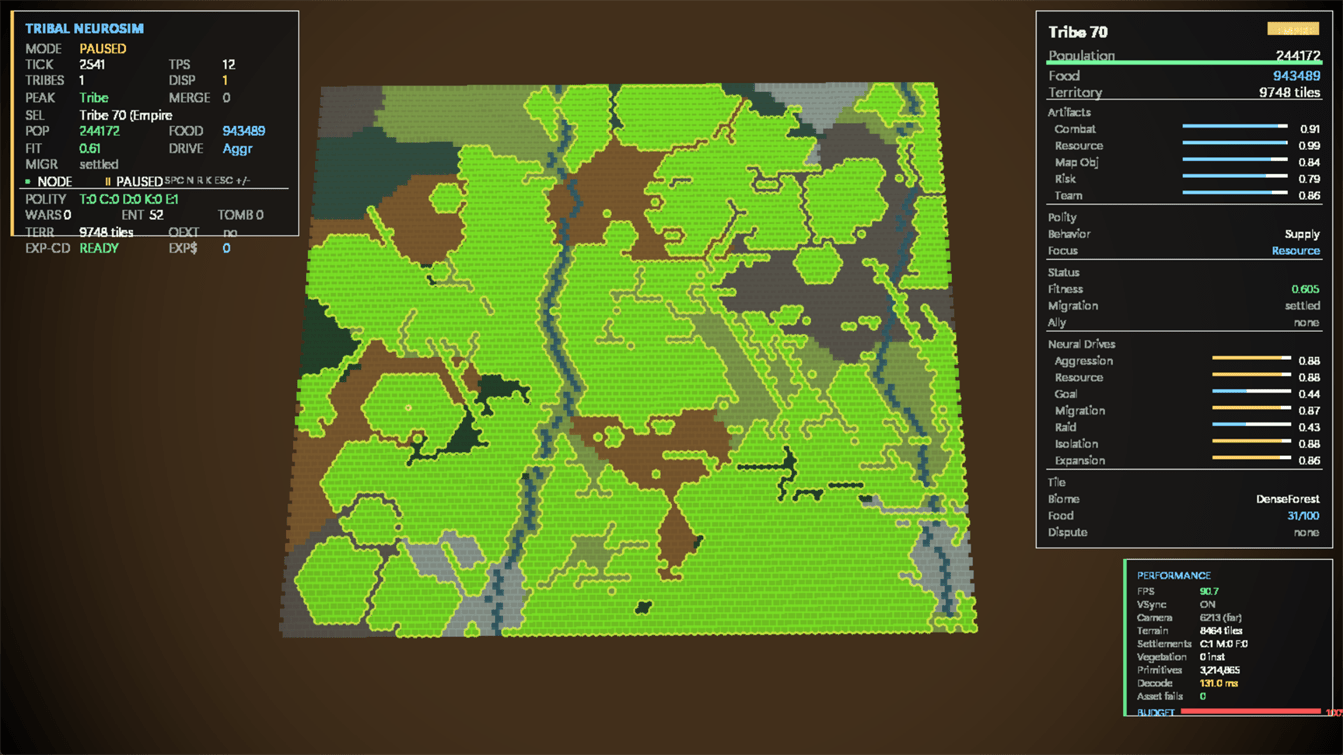
\includegraphics[width=0.9\textwidth]{assets/neurosim/run67sq7777-sq-s7777-tick2541-last.png}
\caption{SoloQ, seed=7777, tick=2541: Tribe 70 (Supply/Resource) győzelme, 9\,748 tile-os végső területtel.}
\end{figure}

\section{103-seed sweep és győztes archetípus-eloszlás}

A négy kísérleti futtatást egy 103 seed alapú soloq sweep egészíti ki. A sweep minden futtatása Empire polity-szintű győztessel zárult (103/103). Az archetípus-eloszlás:

\begin{table}[H]
\centering
\caption{Győztes archetípus-eloszlás a soloq 103-seed sweep alapján}
\label{tab:soloq-sweep-archetypes}
\begin{tabular}{lrr}
\toprule
\textbf{Archetípus} & \textbf{Futtatások} & \textbf{Arány} \\
\midrule
Warband   & 36 & 35{,}0\% \\
Supply    & 23 & 22{,}3\% \\
Council   & 20 & 19{,}4\% \\
Vanguard  & 14 & 13{,}6\% \\
Pathfinders & 10 & 9{,}7\% \\
\midrule
\textbf{Összesen} & 103 & 100\% \\
\bottomrule
\end{tabular}
\end{table}

Az átlagos befejezési tick 2308{,}57; az átlagos győztes terület 8\,338 tile. A Warband archetípus enyhe pluralitással vezet (35\%), de nem rendelkezik erős, seed-független dominanciával.

\section{Adatkészlet-összehasonlítás és értelmezési határok}

A két tesztelt flexset futtatás (seed=42 és seed=7777) mindkét esetben Warband/Combat profilú entitás győzelmével zárult, alacsony agresszióval (0{,}13--0{,}18) és magas migrációval (0{,}87--0{,}88). A soloq futtatások változékonyabb győztes-profilt produkáltak: seed=42 Vanguard/Risk, seed=7777 Supply/Resource győztest hozott.

Ez a különbség a mögöttes gráfstruktúrából értelmezhető. A flexset adatkészlet szervezettebb, ismétlődő kapcsolatmintákat hordoz, míg a soloq adatkészlet inkább egyéni teljesítményprofilokat rögzít tartós co-queue struktúra nélkül.

Az értelmezés korrelatív, nem okozati. A determinisztikus batch-ellenőrzés helyességét igazolta: flexset seed=42 esetén öt párhuzamos fejnélküli futtatás mindegyikében Tribe 596 (Warband/Combat) győzött, bit-azonos \textit{final\_summary} rekordokkal.

Az eredmények alátámasztják, hogy a klaszter-derivált priorok mérhetően eltérő szimulált viselkedést produkálnak azonos szabálykörnyezetben. Az eredmények nem bizonyítanak valódi játékos-pszichológiát és nem adnak előrejelzést tényleges League of Legends meccsek kimenetelére.
